% ----------------------------------------------------
% Firmware Submodule
% ----------------------------------------------------
\chapter{Firmware development \label{ch:firmware}}
\section{Subsystem introduction}

This subsystem deals with the development of firmware for the microcontrollers in both the camera/transmitter and receiver modules. The fundamental goals of this subsystem are to enable the camera/transmitter module to take photographs of the red-winged starlings, and to transmit this photographs to the receiver module without disturbing the birds' nests. The source code for this subsystem is available in the \href{https://github.com/rothdu/EEE4113F-Group13-2024}{project repository} on GitHub.

Section \ref{s:firmware-requirements} presents a traceability matrix with the subsystem's user requirements, interpretted functional requirements, and the corresponding ATPs. Section \ref{s:firmware-design-decisions} discusses high-level design decisions that informed the subsystem development process. Section \ref{s:firmware-design-process} details the design process and the functionality of the final implementation. Finally, section \ref{s:firmware-atps} shows the acceptance test procedures, proving that the user requirements have been adequately met.

\section{Requirement analysis} \label{s:firmware-requirements}
User requirements where determined from discussions with the red-winged starling researchers \cite{hofmeyer2024private}. The user requirements were interpretted to form functional requirements for the subsystem, and an acceptance test was developed for each requirement. The traceability matrix displaying the requirements is shown in Table \ref{tab:firmware-requirements}.

\centering
\begin{longtable}{|p{0.3\textwidth}|p{0.5\textwidth}|p{0.1\textwidth}|}
    \hline
    \textbf{User requirement} & \textbf{Functional requirement} & \textbf{ATPs} \\ \hline
    Triggered with movement & Image must capture fast enough to see the object that triggered the movement & ATPs \\ \hline
    Data access without disturbing nests & A wireless communication protocol must be set up to transfer camera/transmitter data to the receiver & ATP \\ \hline
    Repeated photographs or video footage & Camera must capture multiple time per trigger or take video footage & ATP \\ \hline
    Access to images in real time & Tranmission from the camera/transmitter module must be available on-demand from the receiver module, or triggered daily in autonomous mode & ATP \\ \hline
    Data gathering over 7-week breeding season without frequent camera/transmitter battery changes & Camera/transmitter module must utilise power-saving modes where possible & ATP \\ \hline
    Uncertainty about required image quality and trigger frequency & Camera/transmitter module must include remotely updateable configuration options & ATP \\ \hline
    Deployment of multiple camera/transmitter modules for different nests & Receiver device must handle separate image storage and configuration options for many camera/transmitter modules & ATP \\ \hline
    \caption{Requirement analysis traceability matrix for firmware subsystem}
    \label{tab:firmware-requirements}
\end{longtable}
\raggedright


\section{High-level design decisions } \label{s:firmware-design-decisions}

This section details high-level design decisions that were made prior to any implementation and testing. These decisions determined key aspects of the development process.

\subsection{Development environment}


\begin{table}[ht]
    \resizebox{\textwidth}{!}{%
    \begin{tabular}{|l|l|l|l|l|}
    \hline
    \textbf{Device}                      & \textbf{Environment}        & \textbf{Library support} & \textbf{Online support/userbase} & \textbf{Abstraction level} \\ \hline
    \multirow{4}{*}{ESP32}               & \textit{C/C++ with ESP-IDF} & \color{red}Adequate                 & Moderate (professional)          & Close to hardware          \\ \cline{2-5} 
                                         & \textit{Arduino}            & Extensive and adequate   & Extensive (hobbyist)             & Somewhat abstracted        \\ \cline{2-5} 
                                         & \textit{MicroPython}        & More limited             & Minimal (hobbyist)               & Very high-level            \\ \cline{2-5} 
                                         & \textit{CircuitPython}      & More limited             & Minimal (hobbyist)               & Very high-level            \\ \hline
    \multirow{5}{*}{Raspberry Pi Pico W} & \textit{Native C/C++ SDK}   & Adequate                 & Moderate (professional)          & Close to hardware          \\ \cline{2-5} 
                                         & \textit{Official Arduino port}          & Adequate                 & Moderate (hobbyist)              & Somewhat abstracted        \\ \cline{2-5} 
                                         & \textit{Community Arduino port}          & Adequate                 & Moderate (hobbyist)              & Somewhat abstracted        \\ \cline{2-5} 
                                         & \textit{MicroPython}        & Extensive and adequate   & Extensive (hobbyist)             & Very high-level            \\ \cline{2-5} 
                                         & \textit{CircuitPython}      & Adequate                 & Moderate (hobbyist)              & Very high-level            \\ \hline
    \end{tabular}%
    }
    \caption{Summary of common coding environments for the available microcontroller}
    \label{tab:coding-env}
    \end{table}

Both available microcontrollers support a variety of code development environments, including their own native C/C++ with available developer libraries, Arduino, MicroPython and CircuitPython.A summary of the support and features of the various coding frameworks is presented in Table \ref{tab:coding-env}.

Coding both microcontrollers using the same framework is a key consideration. This makes the code development process easier both in the current iteration of the project, and for a future engineer who may wish to modify the code, as it requires knowledge of only one framework. 

Low-level C/C++ frameworks are used extensively in professional settings for both microcontrollers. The low-level access to hardware can allow advanced configuration of the microcontrollers. However, low-level development tends to be more complex than development using abstracted frameworks. The low-level hardware access was not necessary for the development of this project, and the easier code development of more abstracted environments was thus preferred.

Of the abstracted languages, Arduino has the most library and online user support for the ESP32, while MicroPython has the most support for the Raspberry Pi Pico W.

Arduino was ultimately chosen as the framework for both microcontrollers. The ESP32 in this project requires more complex functionality and was thus prioritised in terms of library and online support. Furthermore, although Arduino is not necessarily well supported on the Pi Pico W specifically, the framework itself has significant online support, and the library support was deemed adequate for this project.

\subsection{File transfer method}

Both the receiver and transmitter modules support WiFi and Bluetooth. Both protocols are suitable for file transfer in the right circumstances.WiFi was selected as the optimal solution for the following reasons:
\begin{itemize}
    \item Superior range
    \item Superior transfer speeds
    \item Ability to connect to existing network on campus
\end{itemize}

A more extensive breakdown of this choice is described in %TODO reference to Thiyashan's section

Numerous file transfer protocols exist, including encrypted and unencrypted protocols. A secure protocol was not necessary for this application, as the device does not transmit sensitive data. The encryption involved inherently makes them more complex and often less efficient; as such, only unencrypted protocols were considered.

Standard unencrypted protocols include User Datagram Protocol (UDP), Tranmission Control Protocol (TCP), File Transfer Protocol (FTP) and Hypertext Transfer Protocol (HTTP). UDP and TCP are low-level protocols; using a standard higher-level prtocol such as FTP or HTTP is more appropriate unless very fine control of data transmission is needed. Of FTP and HTTP, HTTP is more widely supported and thus easier to implement. It is well supported through standard Arduino libraries.

https://github.com/xreef/SimpleFTPServer

\subsection{Server and client location}

Communication over HTTP is based on a client-server model, where a client sends a request to a known host. It was decided that the camera/transmitter module would act as the client, while the server would be hosted on the receiver, or on a personal computer. 

The server requires a known IP address such that the client knows where to direct it's requests. Once a client has connected to the server, the server sends it's response directly back to whatever client responded to it. The network settings of the UCT campus WiFi do not allow devices to set static IP addresses, meaning it is impossible to host the server on the campus WiFi. If the camera/transmitter acts as the client, it does not need a known IP address when connected to campus WiFi, and could connect to a remotely hosted server. Aditionally, hosting the server on the receiver device allows for traditional web browsers to remotely connect as a client for applications such as updating configuration settings (which could then be pushed to the camera/transmitter module upon request). Finally, a client model is able to make a request to a server immediately, whereas a server must wait for the client to initiate a connection. To save power on the camera/transmitter module, it was useful to allow the module to immediately initiate connection to the server by acting as the client.

\subsection{Library selection}

The Arduino framework includes a wide variety of software libraries. These include "standard" libraries, which are integrated into the Arduino framework or the Arduino core for a particular device, and user-supplied libraries which are uploaded by Arduino users. In most cases, the "standard" libraries have the best support and documentation, and are known to be relatively bug-free; as such, "standard" libraries were used for all applications for which they were available.

Some specific library selections falling outside of this general principle were:

\begin{itemize}
    \item ArduinoJson cites 10\% better speed and memory efficiency than the "standard" library, and has extensive documentation available on its website.
    \item ScreenUI  is a user-implemented library for easy development of menus which display on LCD screen, which was applied to the receiver module.
    \item Reference I2C library here...
\end{itemize}

% TODO: reference the libraries I've used



\section{Submodule design} \label{s:firmware-design-process}

\subsection{High level camera/transmitter module firmware flow}

\begin{figure}[ht]
    \centering
    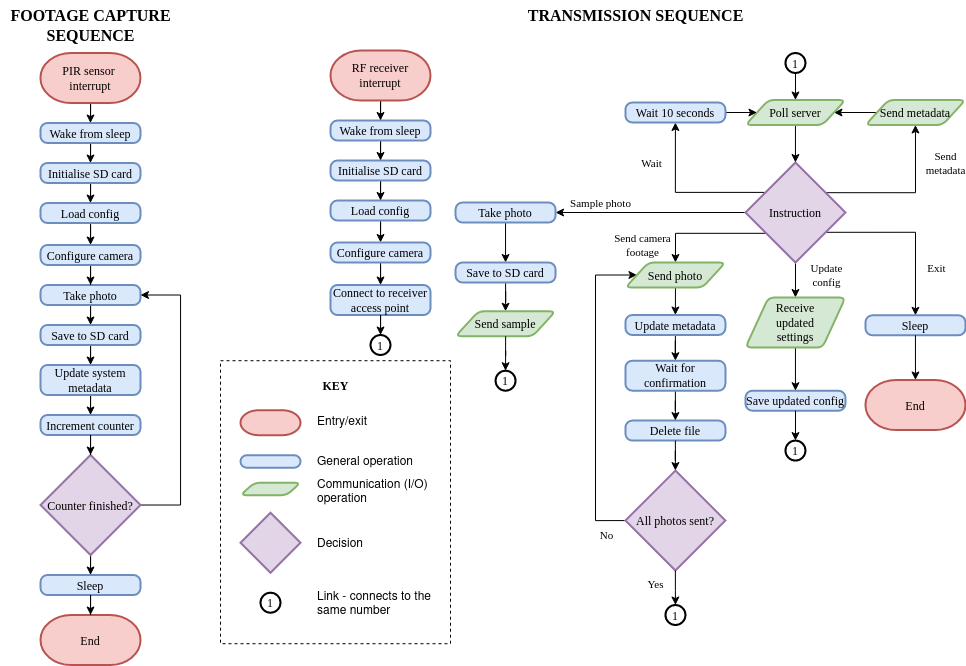
\includegraphics[width=\columnwidth]{"Images/ESP-flow.png"}
    \caption{Flowchart representing the program flow of the ESP32 Camera/Transmitter module}
    \label{fig:espflow}
\end{figure}

Figure \ref{fig:espflow} demonstrates a high-level program flow of the Camera/Transmitter module. The two sequences operate independently and are capable of executing in parallel, by leveraging the dual cores of the ESP32 and the FreeRTOS tasks. The module has two primary purposes - capturing footage, and transmitting it. Transmission can be triggered manually from the reveiver module, with an interrupt that comes via the RF receiver. Otherwise, if the module is configured to act in permanent station mode, the transmission sequence will activate once daily, or when the SD card is 80\% full.

\subsection{HTTP server API}

The HTTP server implemented on the receiver module or a standalone computer must have available endpoints for all the applications the client wishes to utilise.

\subsection{Camera/transmitter module configuration file}

To meet the identified soft-configurability requirement, the ESP32 module will read a customiseable configuration file to determine a number of key settings. The configuration file is stored in plaintext json at "starling-cam/config/config.json" on the microSD card. If the configuration file is unavailable or unreadable, or any configuration parameters are invalid or missing, any missing parameters are loaded as defaults.

This configuration option has a number of advantages:

\begin{itemize}
    \item Storing configuration on the microSD card makes it possible to load new configuration options without needing to flash new code onto the ESP32 or access it remotely.
    \item JSON is human-readable format, making easily possible to write new configuration files.
    \item JSON is a well-supported format, and can easily be read and interpretted on the ESP32 using the ArduinoJson library % TODO \ref{arduinoJSON ref here}
\end{itemize}

\subsection{Camera sensor settings}

The user requirements specified that video or image capture was acceptable, though for the latter a number of images in quick succession would be preferable. A key limitation in this regard was the microSD card on the camera/transmitter module, which had to be formatted with the FAT32 filesystem in order for the module to interface with it. FAT32 is an older file system which only supports up to 4GB of storage. This storage limitation made still image capture more feasible, especially allowing for the possibility that images would be captured many time each day.

% TODO: Probably some test about file size and a proper analysis of photo vs video

% TODO: A proper analysis of the settings available

\subsection{Camera speed testing}


\section{Acceptance Tests \label{s:firmware-atps}}

% Things that need to be implemented:
% Receiver:

% \begin{itemize}
%     \item I2C Led display library
%     \begin{itemize}
%         \item %https://github.com/T-622/RPI-PICO-I2C-LCD/tree/main
%         \item %https://github.com/dhylands/python_lcd
%         \item %https://github.com/peterhinch/micropython-async/tree/master/v3/as_drivers/hd44780
%     \end{itemize}
%     \item Pushbutton inputs
%     \item \begin{itemize}
%         \item Seems to be fine on pi pico
%     \end{itemize}
%     \item Writing to SD card
%     \begin{itemize}
%         \item probably just the default arduino SD library
%     \end{itemize}
%     \item Web server and data reception
%     \item RFID transmitter usage
% \end{itemize}

% Camera:
% \begin{itemize}
%     \item Read/write from SD card
%     \item Read PIR sensors
%     \item Read from Camera
%     \item Enable infrared flash
%     \item Read from RF Receiver
%     \item Read temperature \& humidity sensor
%     \item Read mic
%     \item Connect to web server and transmit data
%     \item Transmit data via direct wifi connection
% \end{itemize}

% Leaning towards Arduino for both - puts the whole project under the same umbrella which would theoretically be useful for future development.
% Might be more limited in bare-metal functionality than ESP-IDF, but should be adequate to get the job done. This is not a time-critical application, so it makes sense to go with an option that makes things easy

% %https://github.com/earlephilhower/arduino-pico
% %https://github.com/arduino/ArduinoCore-mbed
% The second link appears to be the "official" one
% Porting of pi pico SDK to arduino libraries


% Core design decisions:

% \begin{itemize}
%     \item Choice of programming environment {Arduino, python, pi c++, ESP-IDF}
%     \item Choice of Development environment
%     \item How to transmit data (WiFi via HTTP? MQTT? Bluetooth?)
%     \begin{itemize}
%         \item %https://github.com/adafruit/Adafruit_MQTT_Library
%     \end{itemize}
%     \item Library selection
%     \item User interface design
%     \item Upload mode to cloud storage
% \end{itemize}
